\documentclass[14pt]{article}
\usepackage{amsmath}
\usepackage{listings} % For writing code see http://ctan.org/pkg/listings
\usepackage{graphicx}
\usepackage{float}
\usepackage[margin=1.0in]{geometry}
\usepackage{hyperref}

\title{Dynamical model of NGC2419}
\author{Nicolas Garavito-Camargo}
\begin{document}
\maketitle


In this document different dynamical models of \textbf{NGC2419} are explored.


\section{Testing the code:}

A test particle integrated in an NFW profile both with \textsc{Galpy}
and the code developed in this work.

\begin{figure}[H]
\centering
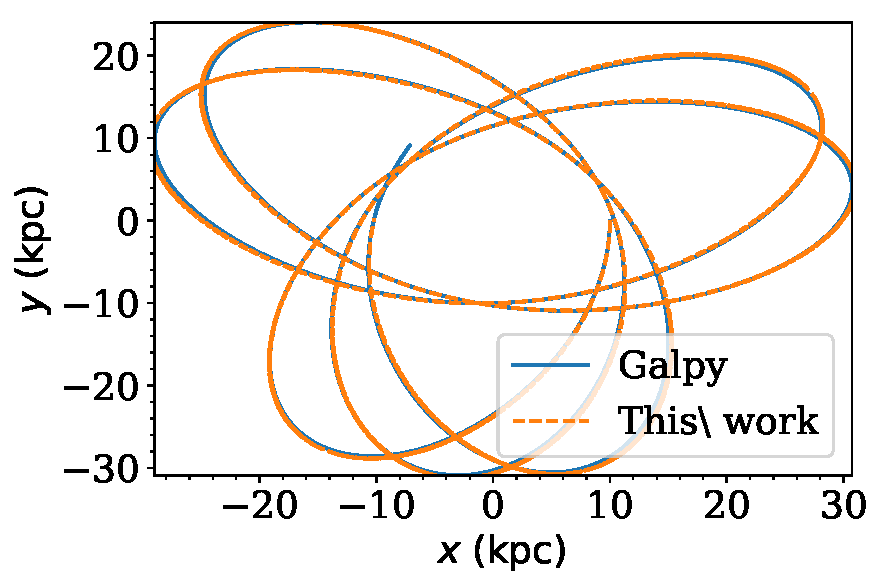
\includegraphics[scale=0.5]{../exploratory_code/galpy_test.pdf}
\end{figure}


\section{The orbit of NGC2419 around the MW}

\begin{table}
\centering
\begin{tabular}{c c c c c}
\hline
\hline
\textbf{Models:} & & & & \\
\hline
Halo: & NFW & $M_{vir} = 1\times 10^{12} M_{\odot}$ & $c=9.86$  \\
Disk: & Miyamoto-Nagai & $M_{d} = 6.5\times10^{10} M_{\odot}$ & $r_L = 3.5 kpc$ & $r_H = 0.53 kpc$ \\
Bulge: & Hernquist & $M_b = 1 \times 10^{10} M_{\odot}$ & $r_s=0.7 kpc$ & \\
\hline
\hline
\end{tabular}
\caption{Milky Way model parameters.}
\end{table}

Using the MW model resumed in table 1 the 

\begin{figure}[H]
\centering
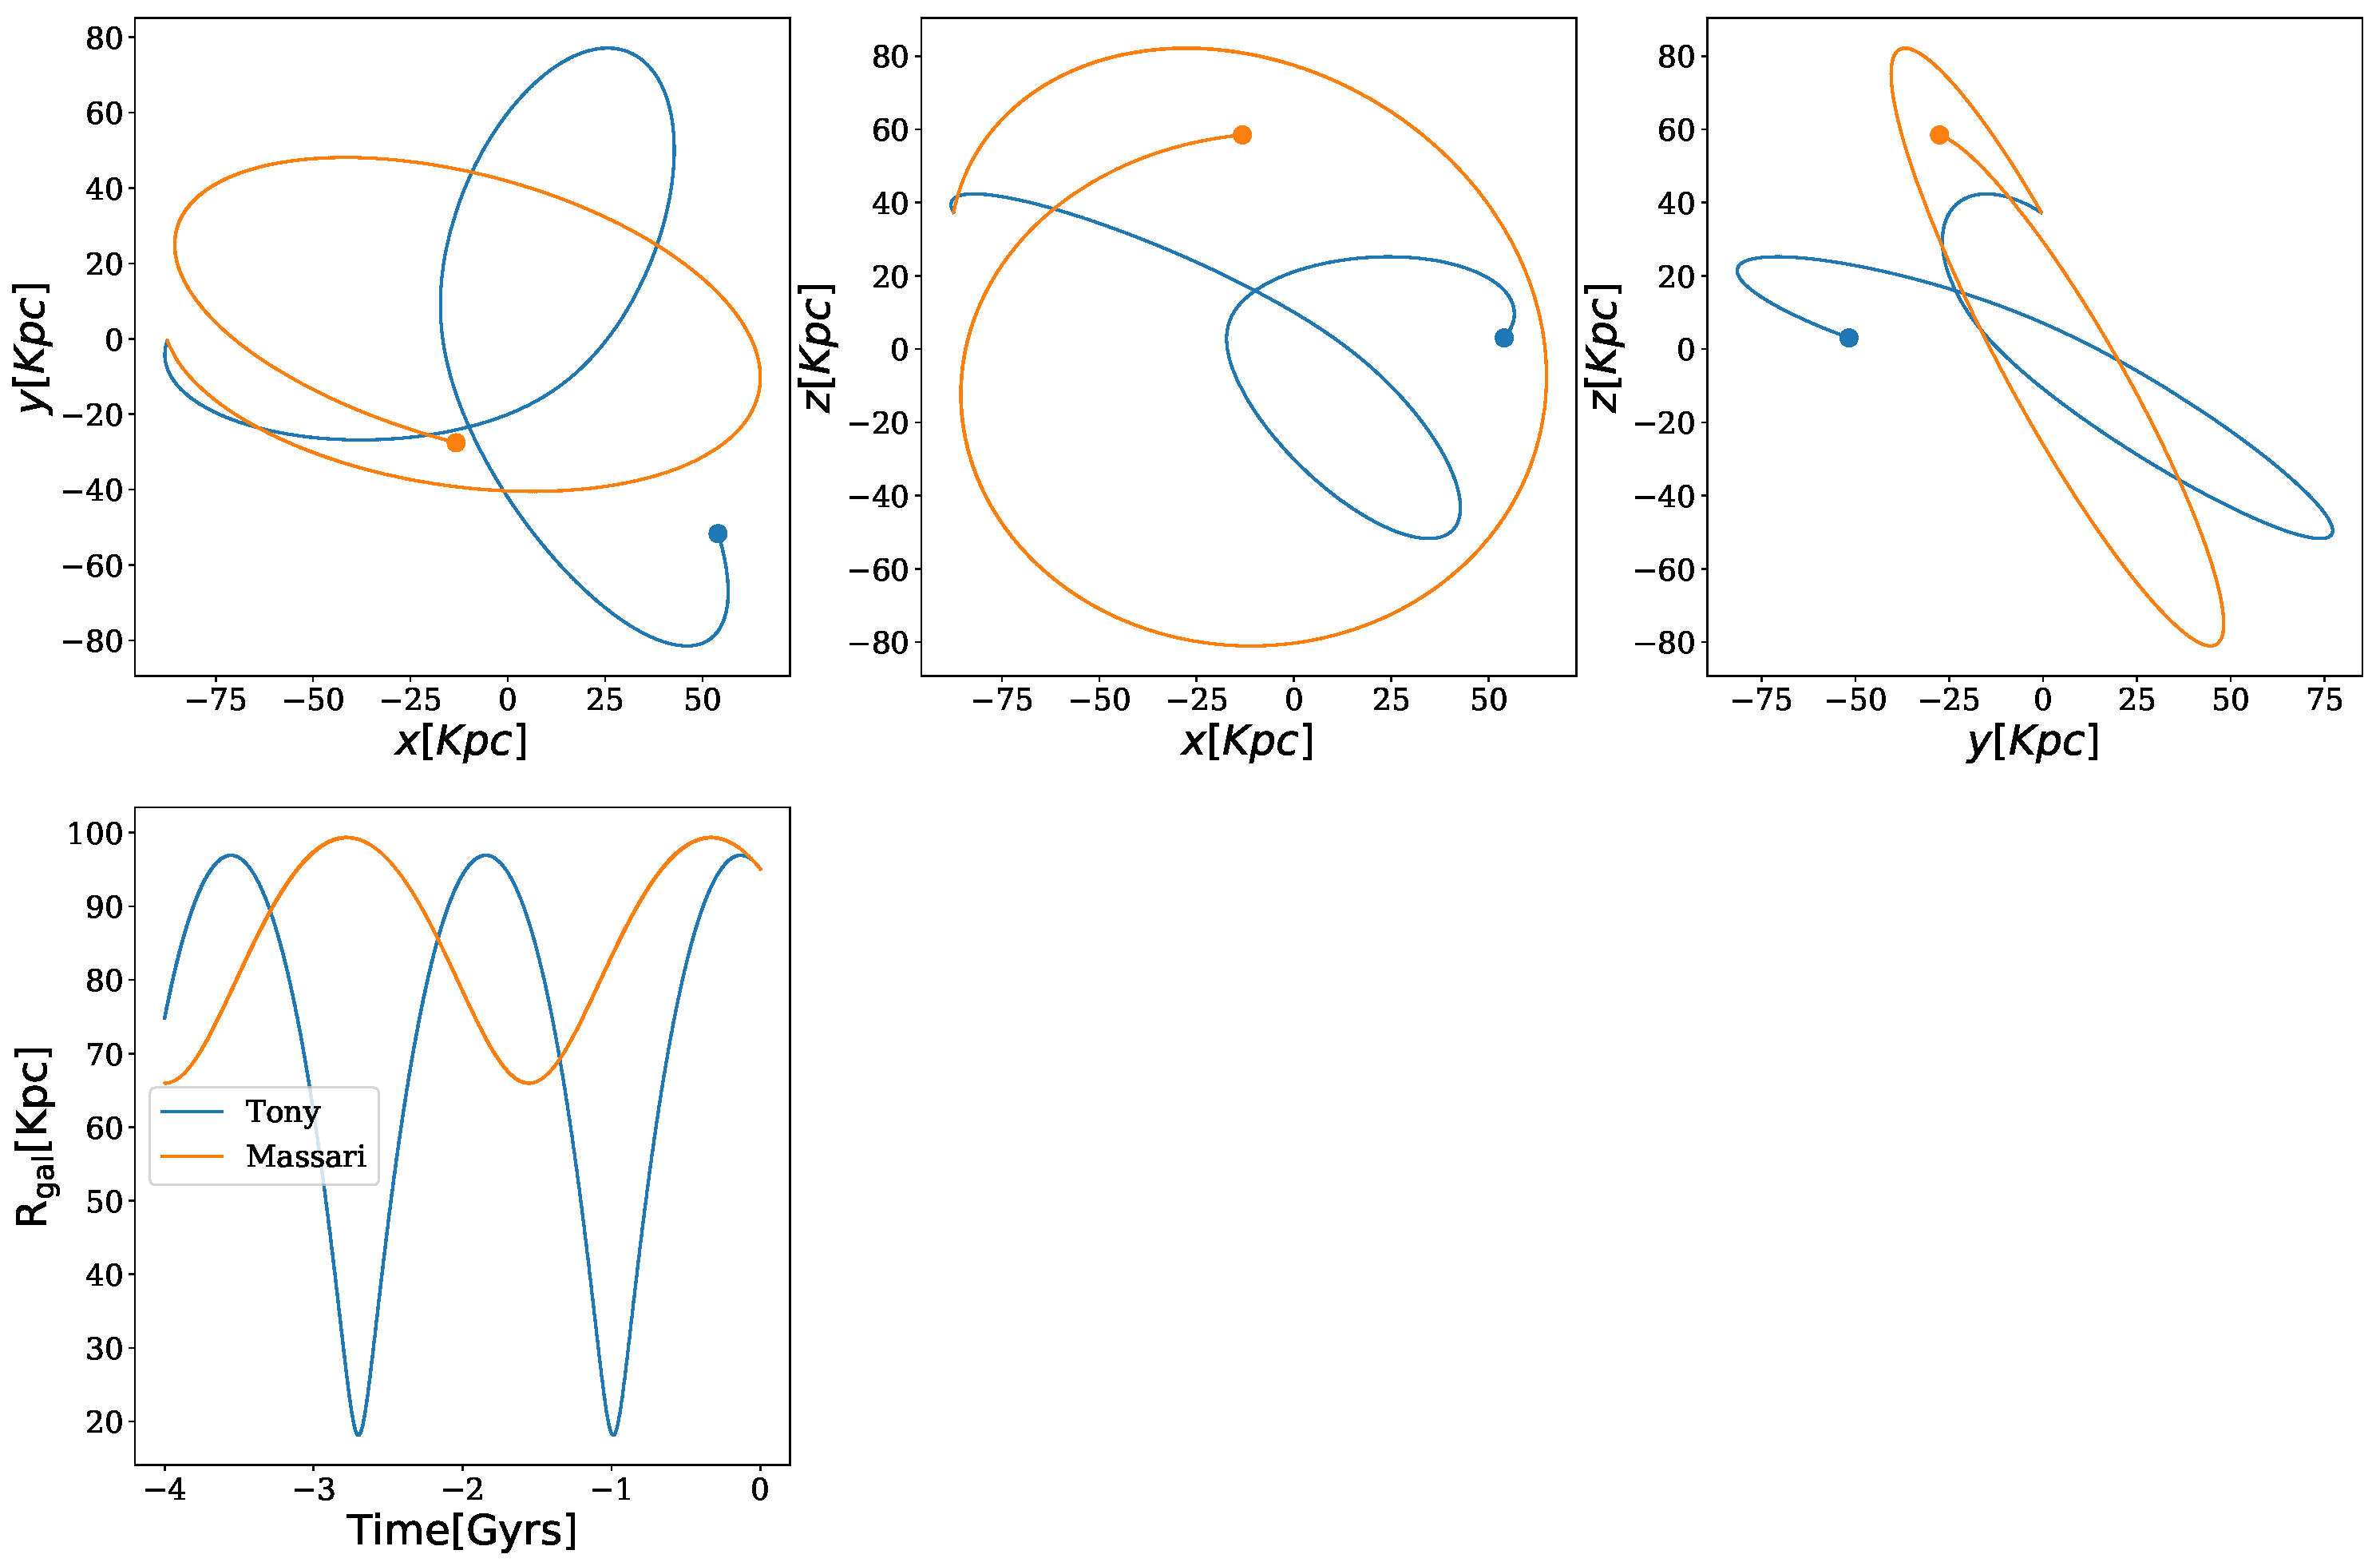
\includegraphics[scale=0.2]{../exploratory_code/NGC2419_sphMW.pdf}
\caption{In a spherical MW halo}
\end{figure}

\begin{figure}[H]
\centering
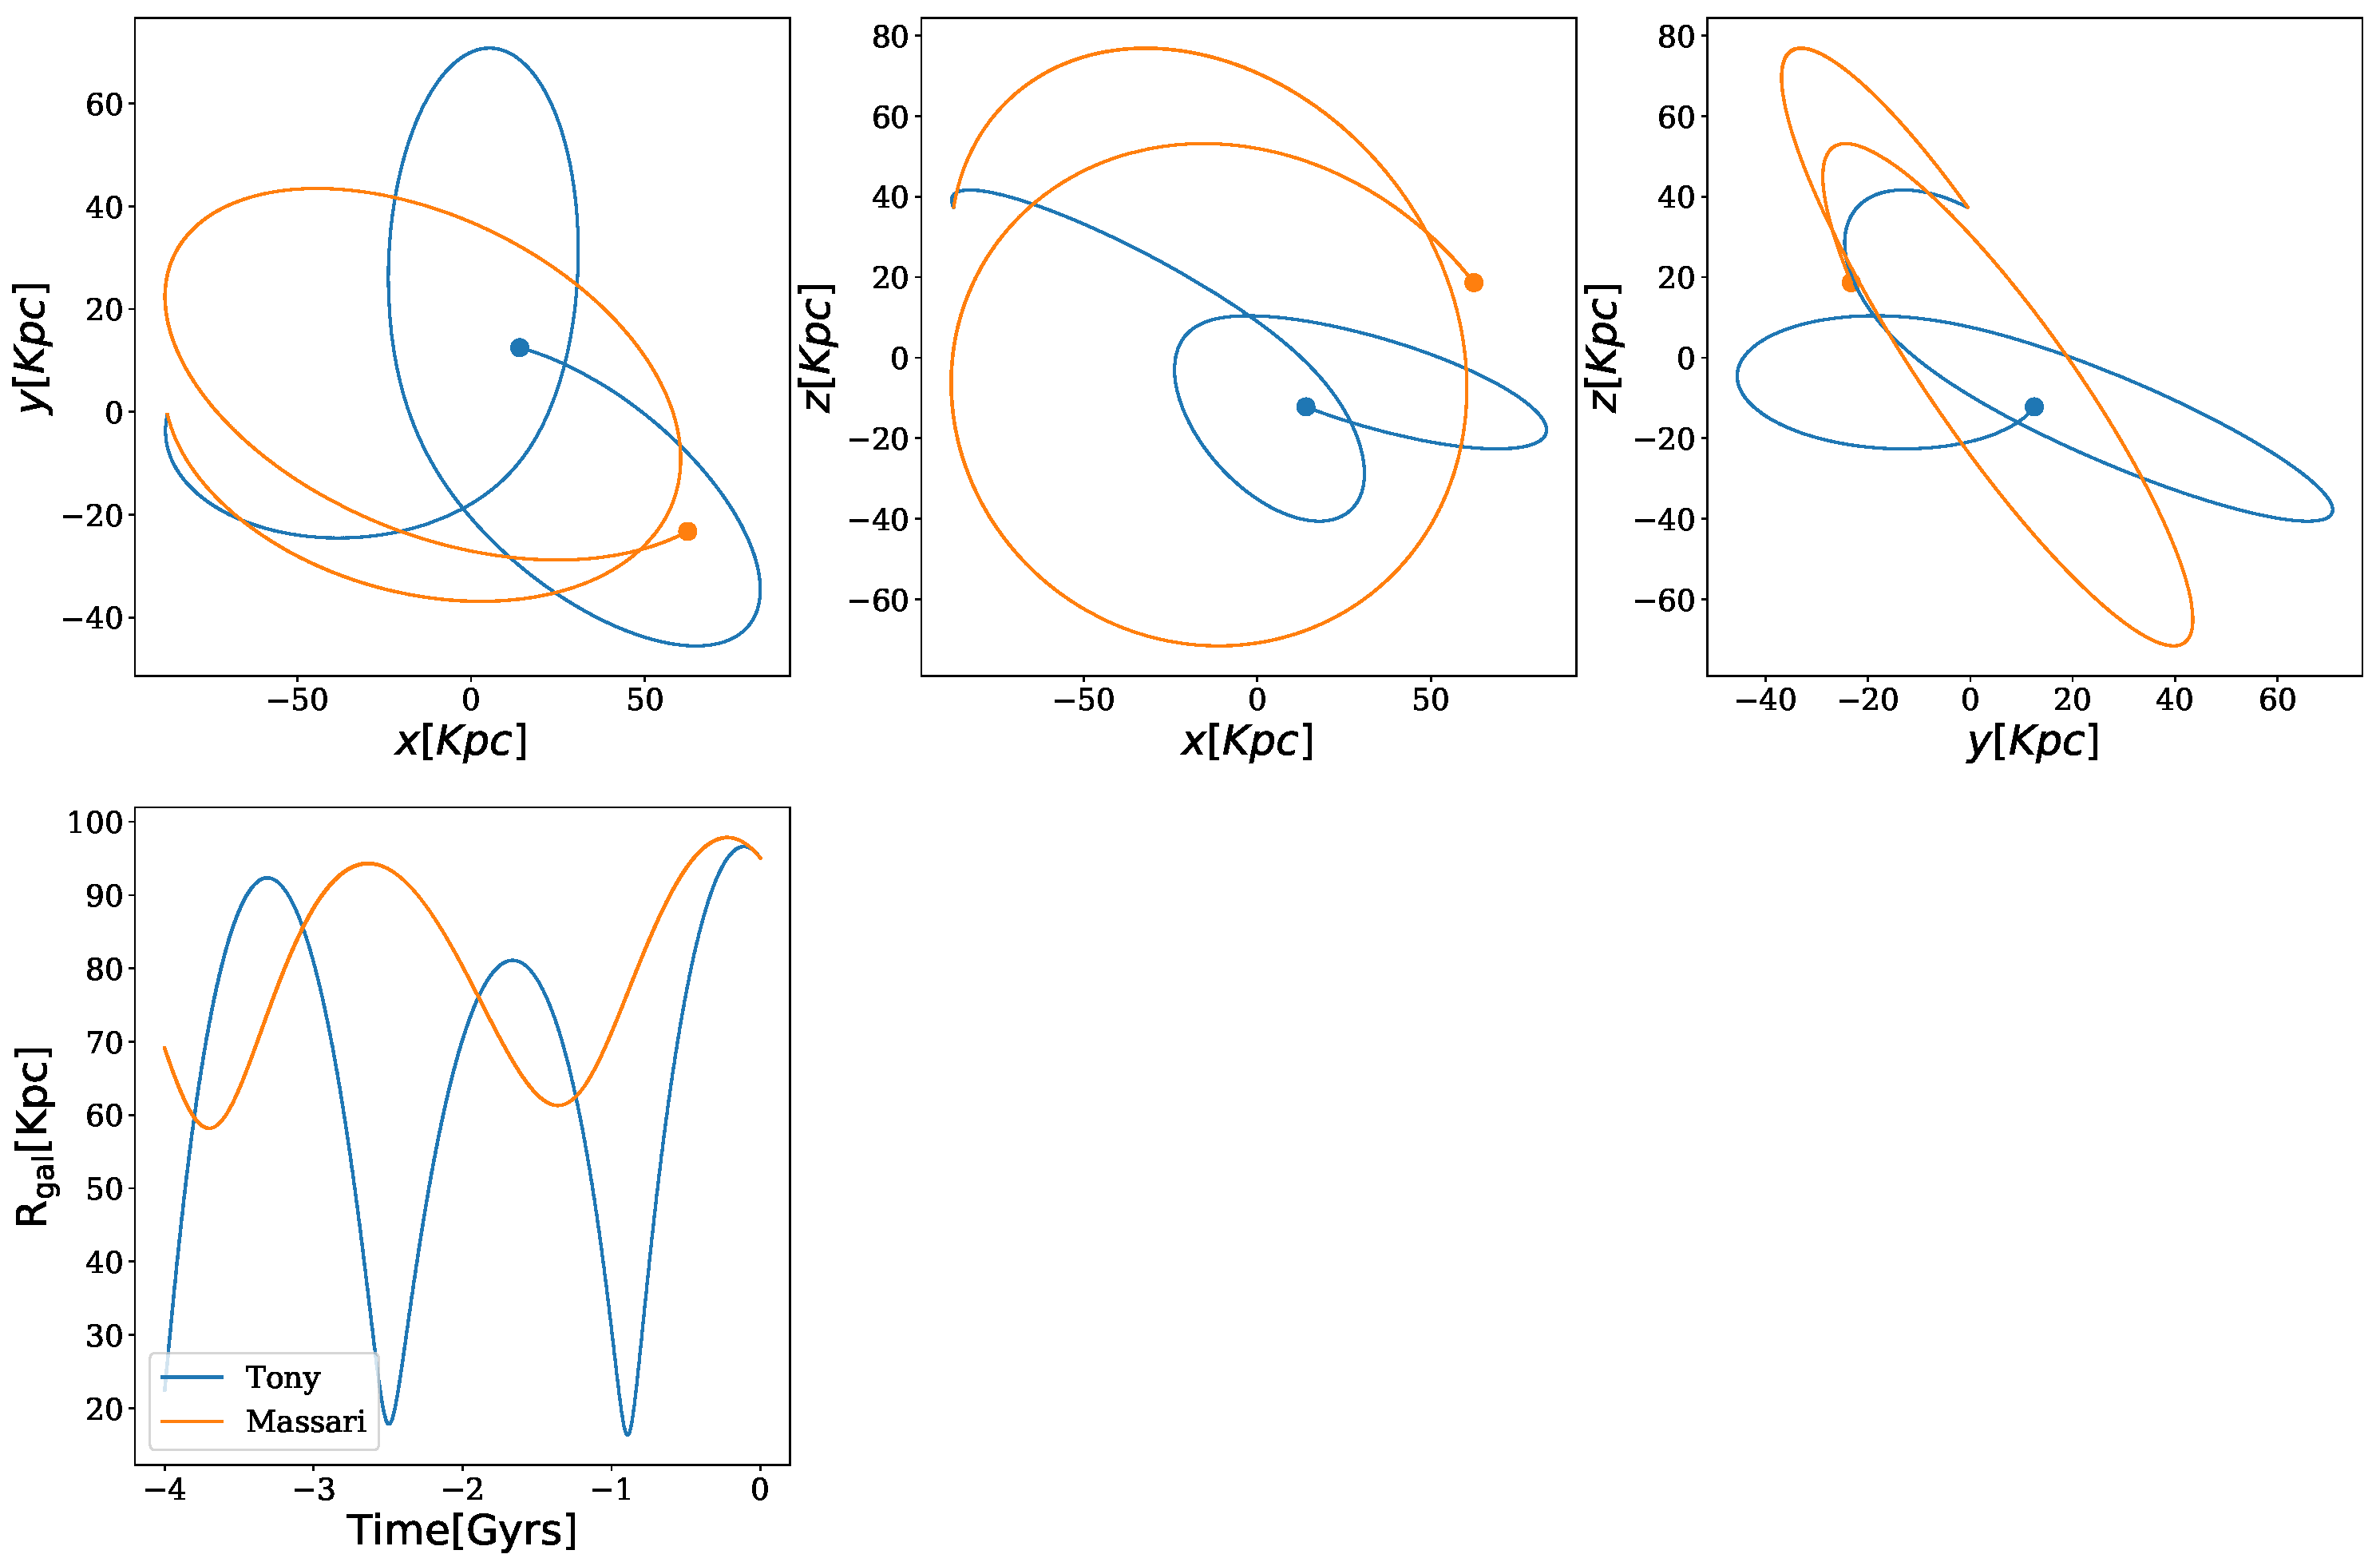
\includegraphics[scale=0.2]{../exploratory_code/NGC2419_Triaxial_MW.pdf}
\caption{In a triaxial MW halo}
\end{figure}

A 3D visualization of this plot can be found 
\href{https://plot.ly/~jngc/3/orbits/?share_key=FcyuVOnd0LYVXaYhGmSuo9}{here}


\section{The orbit of NGC2419 around the MW with Sgr}

Including the Sagittarius (Sgr) dwarf galaxy:


\begin{table}
\centering
\begin{tabular}{c c c c c}
\hline
\hline
Halo: & NFW & $M_{vir} = 1\times 10^{10} M_{\odot}$ & $c=8$  \\
\hline
\hline
\end{tabular}
\caption{Sagittarius dwarf model.}
\end{table}


\begin{figure}[H]
\centering
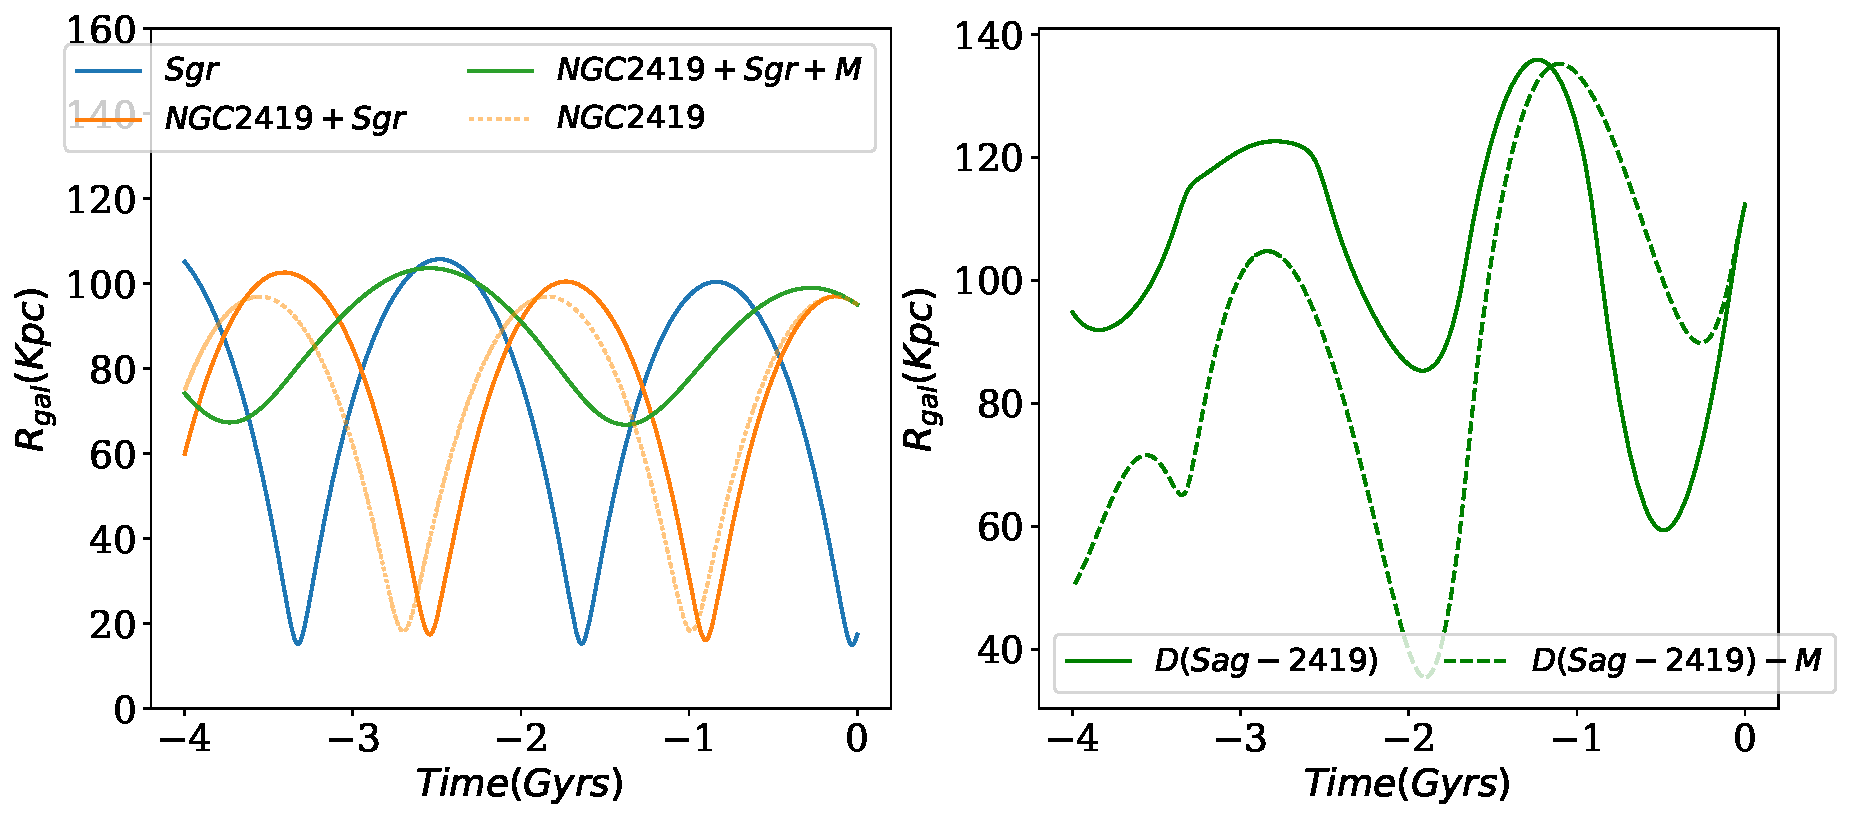
\includegraphics[scale=0.5]{../exploratory_code/NGC2419_sphMWSGR.pdf}
\end{figure}


\section{The orbit of NGC2419 around the MW with Sgr and the LMC}

LMC masses: $[3\times10^{10}, 5\times10^{10}, 8\times10^{10},
1\times10^{10}, 1.8\times10^{11}, 2.5\times10^{11}]$



\begin{figure}[H]
\centering
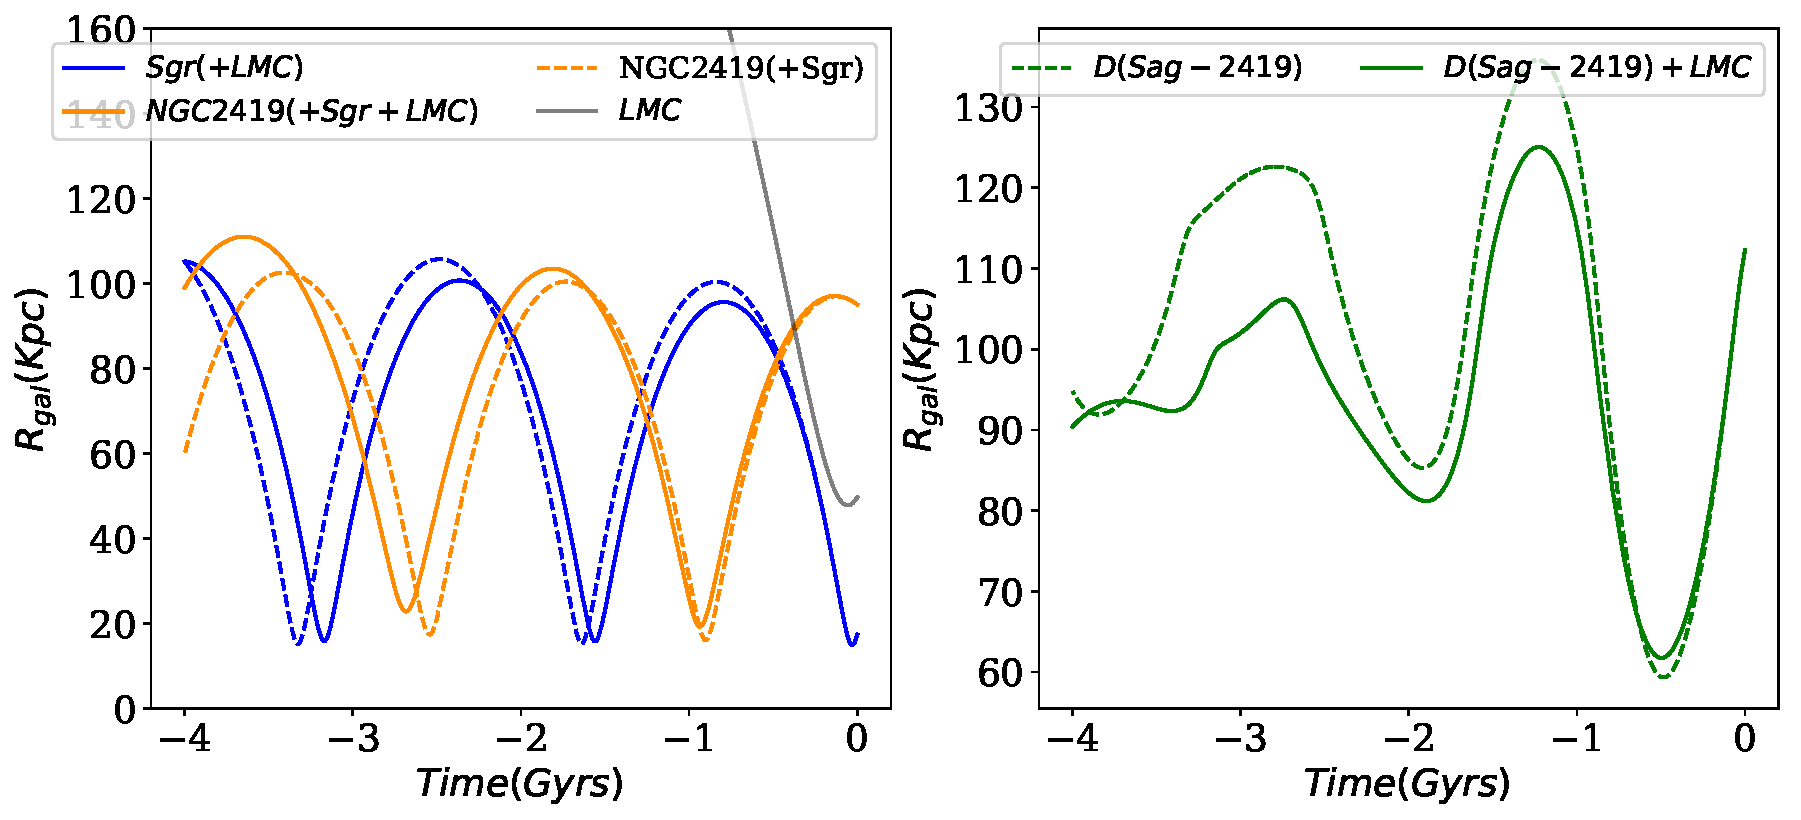
\includegraphics[scale=0.5]{../exploratory_code/NGC2419_sphMWSGRLMC.pdf}
\caption{For the lightest LMC and lightest Sag.}
\end{figure}


\begin{figure}[H]
\centering
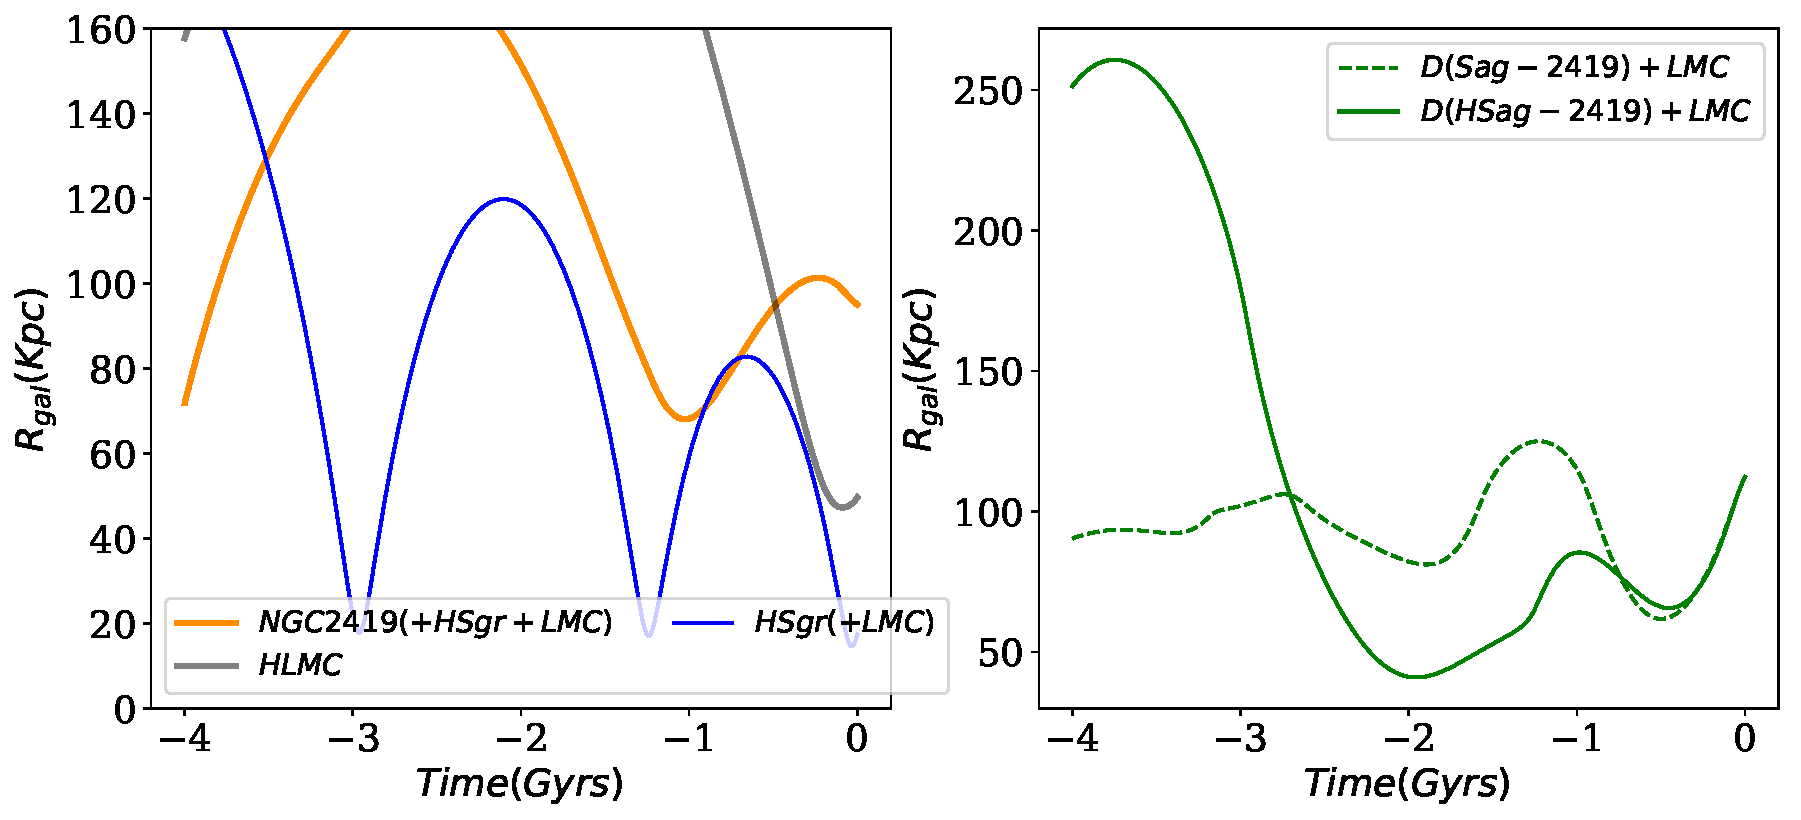
\includegraphics[scale=0.5]{../exploratory_code/NGC2419_sphMWHSGRLMC.pdf}
\caption{for the lightest LMC and Heavy Sag.}
\end{figure}

\begin{figure}[H]
\centering
\begin{minipage}{0.49\linewidth}
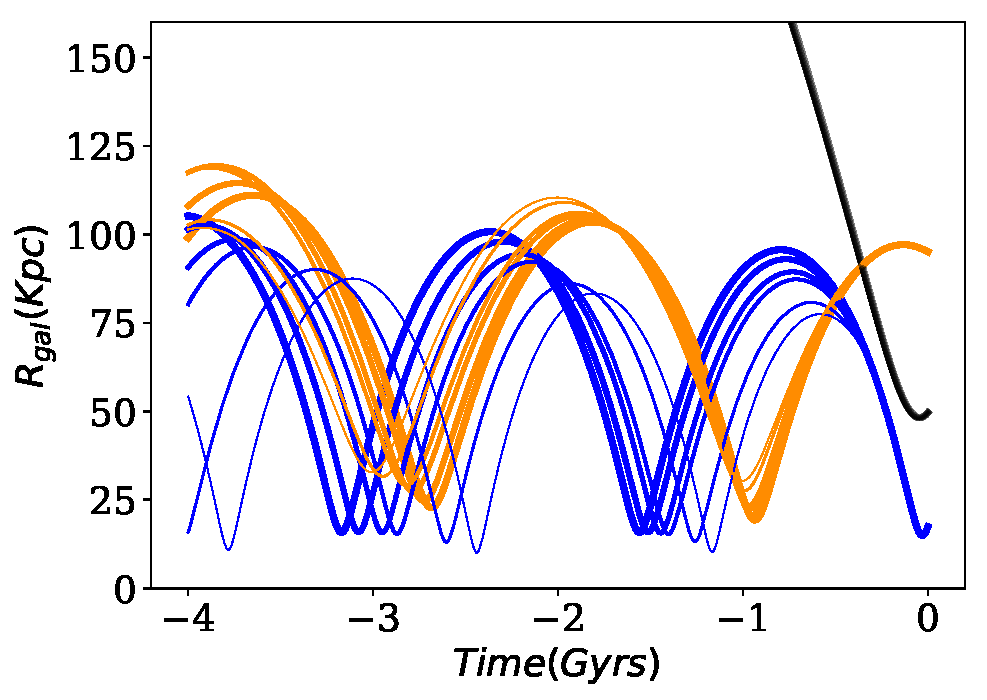
\includegraphics[scale=0.5]{../exploratory_code/gal_orbits_all_LMCs.pdf}
\end{minipage}
\begin{minipage}{0.45\linewidth}
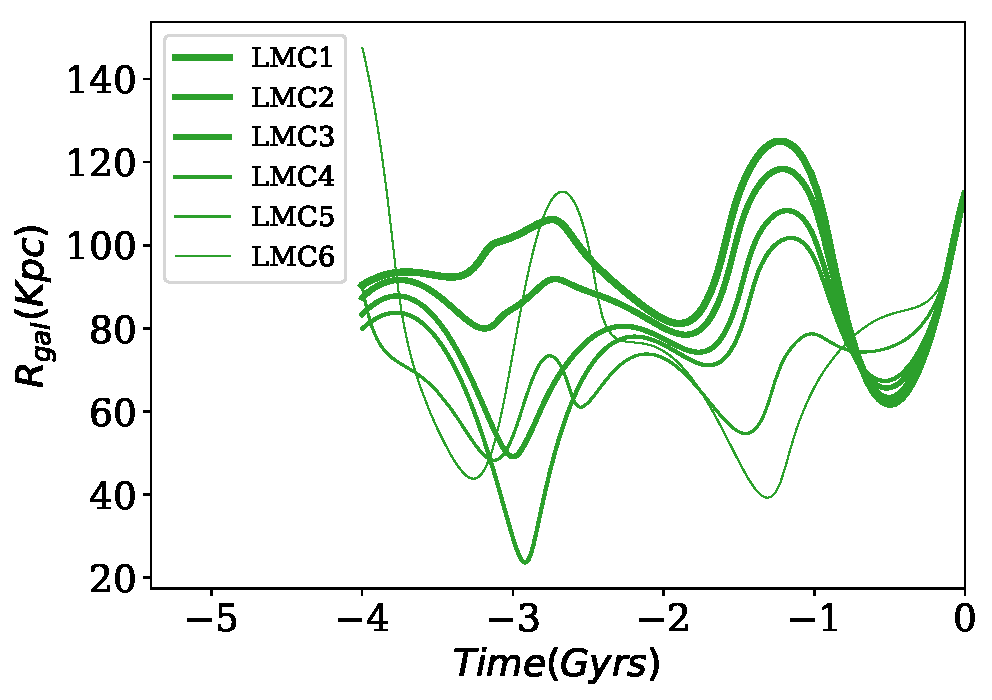
\includegraphics[scale=0.5]{../exploratory_code/d_rel_all_LMCs.pdf}
\end{minipage}
\end{figure}




\begin{figure}[H]
\centering
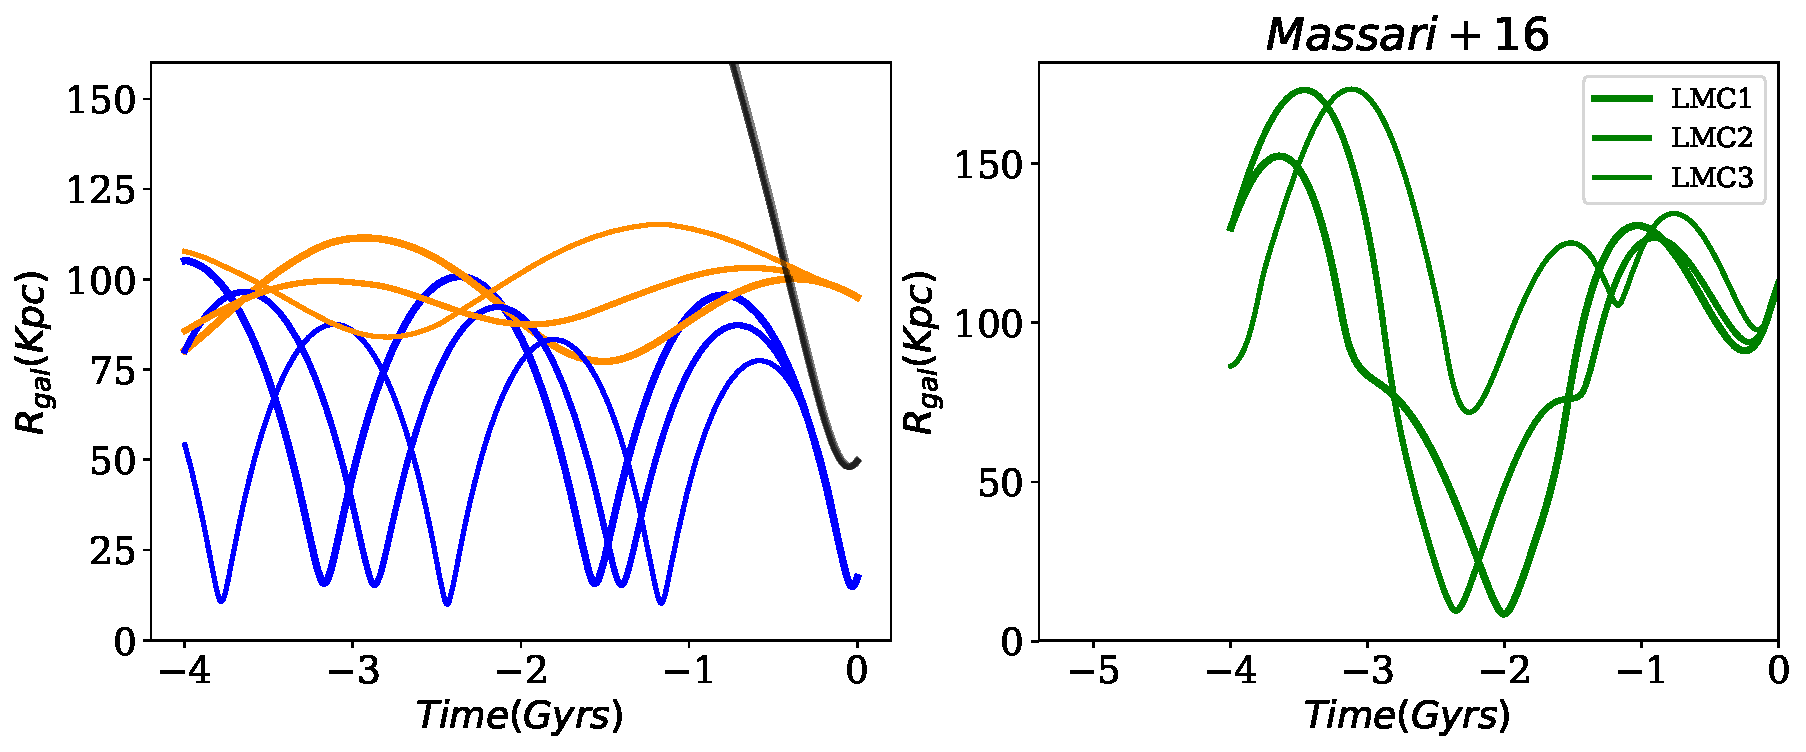
\includegraphics[scale=0.5]{../exploratory_code/gal_orbits_all_LMCs_massari.pdf}
\caption{NGC2419 IC taken from Massari+16 proper motion.}
\end{figure}

\section{The orbit of NGC2419 around the MW in a NFW triaxial
potential with the LMC}


The new potential is a NFW with $c=20$, $q=0.8$ and $s=1$ following
Massari+16.

\begin{figure}[H]
\centering
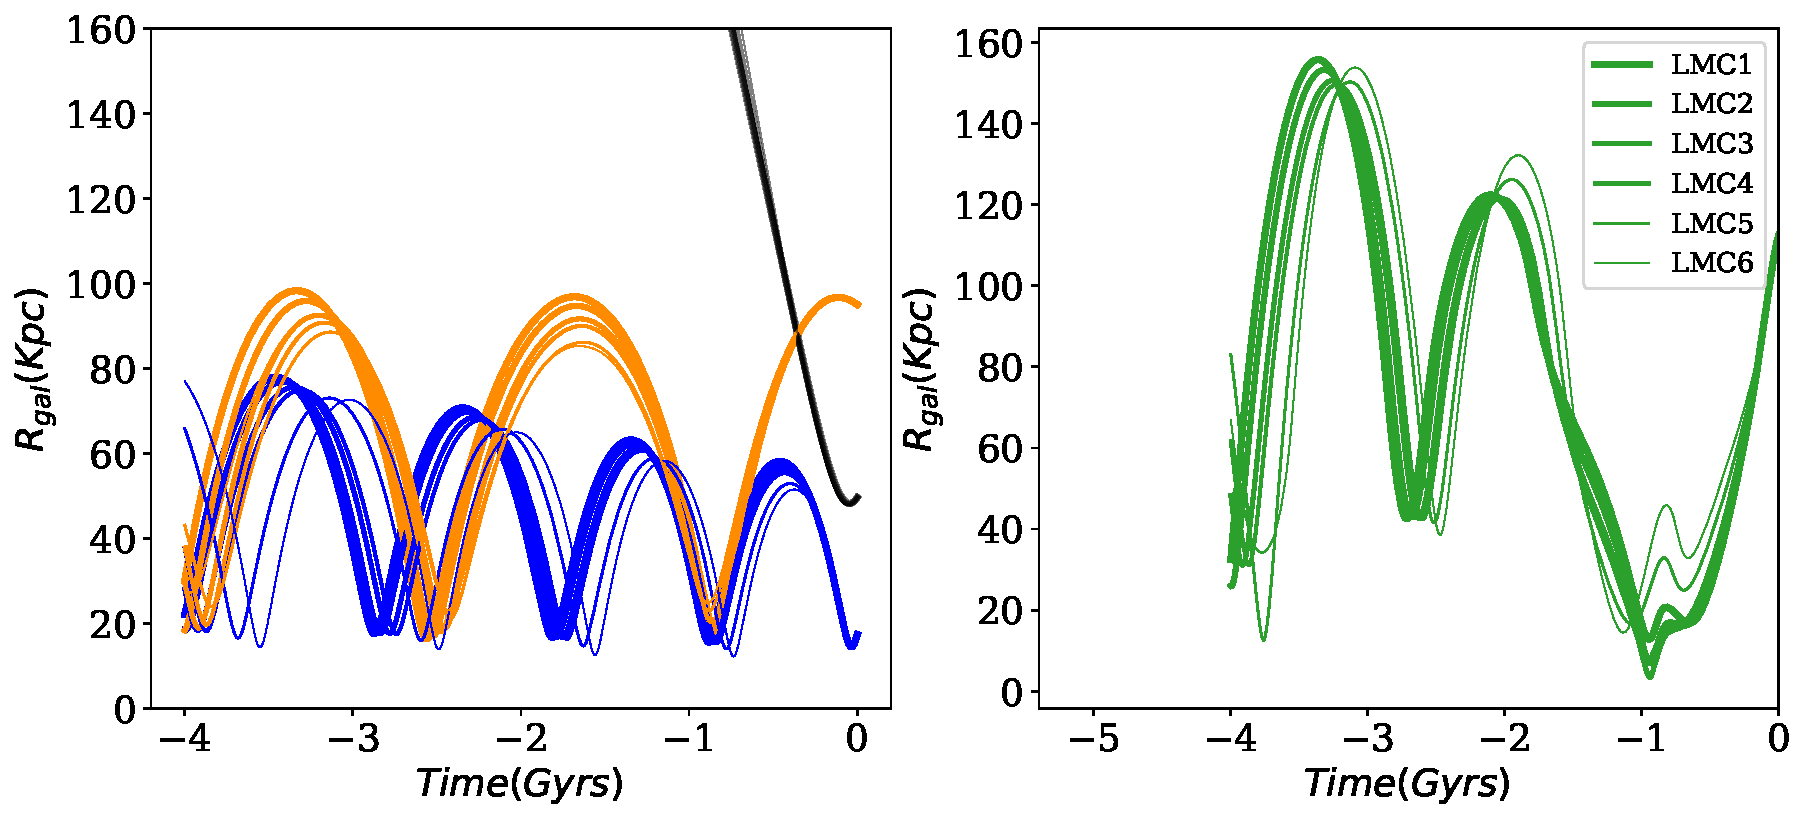
\includegraphics[scale=0.5]{../exploratory_code/gal_orbits_all_LMCs_Triaxial.pdf}
On the right panel the thickness of the line represent a higher mass
LMC
\end{figure}

\begin{figure}[H]
\centering
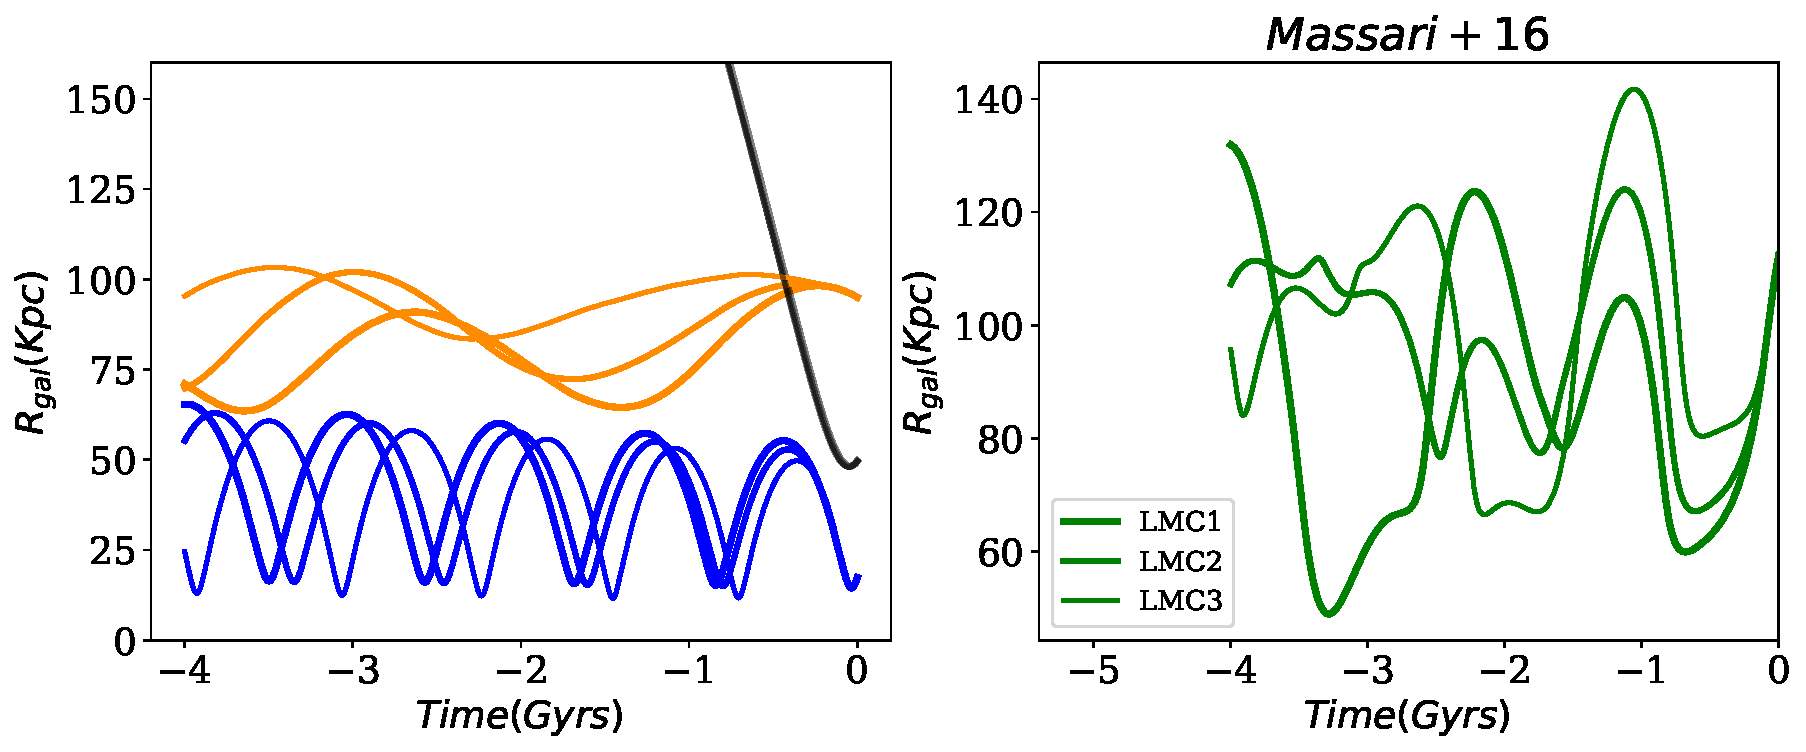
\includegraphics[scale=0.5]{../exploratory_code/gal_orbits_all_LMCs_massari_T.pdf}
\caption{NGC2419 IC taken from Massari+16 proper motion.}
\end{figure}

\end{document}

